\documentclass[12pt,fleqn,leqno,letterpaper]{article}
\usepackage{lmodern}
\usepackage{relsize}
\usepackage[textwidth=7in,textheight=11in]{geometry}% http://ctan.org/pkg/geometry
\usepackage{amsmath, amsthm, amssymb, mathtools}
\usepackage{mathrsfs}

\usepackage{graphicx}
\usepackage{adjustbox}


\title{Homework 8}
\author{Alex Day\\
	\small{Analysis of Linear Systems}
}
\date{\today}

\newcommand{\norm}[1]{\left\lVert#1\right\rVert}

\begin{document}
\maketitle
	\begin{enumerate}
		\item[3a.]
			\begin{align*}
			   &\begin{bmatrix}
				\langle y_{1}, y_{1} \rangle & \langle y_{1}, y_{2} \rangle & \langle y_{1}, y_{3} \rangle \\
				\langle y_{2}, y_{1} \rangle & \langle y_{2}, y_{2} \rangle & \langle y_{2}, y_{3} \rangle \\
				\langle y_{3}, y_{1} \rangle & \langle y_{3}, y_{2} \rangle & \langle y_{3}, y_{3} \rangle \\
				\end{bmatrix}
				\alpha
				\begin{bmatrix}
				\langle y_{1}, x \rangle \\
				\langle y_{2}, x \rangle \\
				\langle y_{3}, x \rangle \\
				\end{bmatrix}\\\\
				\alpha &= \begin{bmatrix} -0.0415 & 0.3518 & -0.9677 \end{bmatrix}^{T}\\
				m_{0} &= \alpha_{1} y_{1} + \alpha_{2} y_{2} + \alpha_{3} y_{3}\\
				m_{0} &= \begin{bmatrix} 0.0461 & 1.2826 & 0.8233 & 0.2227 \end{bmatrix}\\
			\end{align*}
		\item[3b.]
		\item[4a.]
			\begin{align*}
			   &\begin{bmatrix}
				\langle y_{1}, y_{1} \rangle & \langle y_{1}, y_{2}\\
				\langle y_{2}, y_{1} \rangle & \langle y_{2}, y_{2} \\
				\end{bmatrix}
				\alpha
				\begin{bmatrix}
				\langle y_{1}, x \rangle \\
				\langle y_{2}, x \rangle \\
				\end{bmatrix}\\\\
				\alpha &= \begin{bmatrix} 0.9888 & -0.1451 \end{bmatrix}^{T}\\
				m_{0} &= \alpha_{1} y_{1} + \alpha_{2} y_{2}\\
				m_{0} &= \frac{(3360*(\pi^{2} - 10)*t^{3})}{\pi^{7}} - \frac{(240*(2*\pi^{2} - 21)*t)}{\pi^{5}}
			\end{align*}
		\item[4b.]
			\begin{align*}
				\norm{x(\dot) - x_{a}(\dot)}_{2} &\approx 0.00347617397
			\end{align*}
			\begin{minipage}[t]{\linewidth}
				\raggedright
				\adjustbox{valign=t}{%
					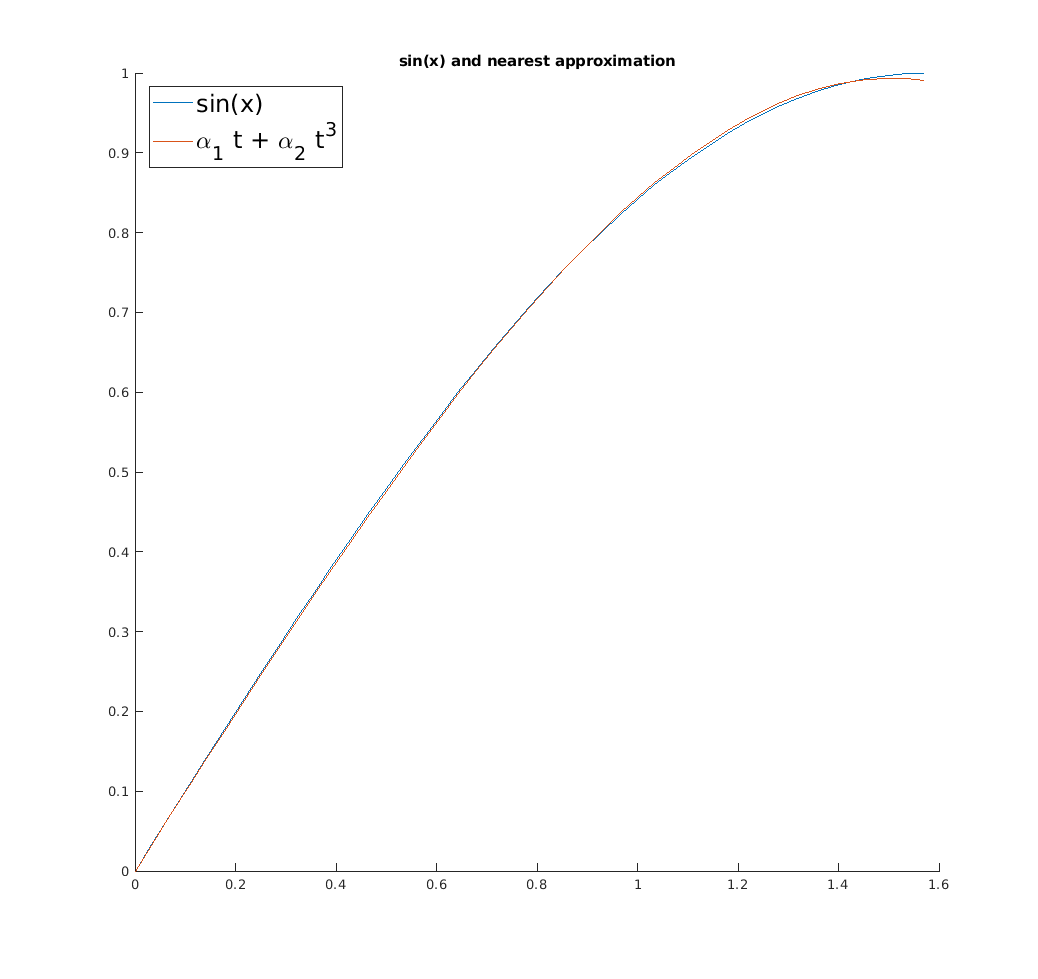
\includegraphics[width=\linewidth]{approx.png}%
				}
				\medskip
			\end{minipage}
		\item[4c.]
			\begin{align*}
				\hat{v}_{1} &= \frac{t}{\norm{t}}\\
				            &= \frac{t}{\sqrt{\pi^{\frac{3}{24}}}}\\\\
				\hat{v}_{2} &= \langle \hat{v}_{1}, y_{2} \rangle v_{1}\\
							&= ( \int_{0}^{\frac{pi}{2}} (\frac{t}{\sqrt{\pi^{\frac{3}{24}}}} t^{3})^{2}  dt) \frac{t}{\sqrt{\pi^{\frac{3}{24}}}}\\
			\end{align*}
	\end{enumerate}
\end{document}
